\section{连续函数}
\label{sec:analysis-local-models}
\label{sec:analysis-metric-continuity-extrema}

\subsection{连续性}

\paragraph{连续函数}
对$f(x)=x^2$，输入$x$接近$a$时，输出$x^2$接近$a^2$，而$a^2$恰好是函数在$a$处的值$f(a)$。连续性描述的就是这种关系：输出趋近的目标等于函数在该点的取值。下面用邻近输入的误差条件表述它；定义域可以是实轴的任意子集，不必是整个区间。
\begin{definition}[连续函数]
\label{def:analysis-continuity}
设$X\subseteq\mathbb R$，$f:X\to\mathbb R$，$a\in X$。若对每个$\varepsilon>0$，都存在$\delta>0$，使
\[
 x\in X,\quad |x-a|<\delta
 \quad\Longrightarrow\quad |f(x)-f(a)|<\varepsilon,
\]
则称$f$在$a$处\term{连续}（continuous）。若$f$在$X$的每一点连续，就称$f$为连续函数。
\end{definition}
定义中的$\delta$可以随$a$和$\varepsilon$改变。连续性与第~\ref{sec:analysis-function-limits}节函数极限的关系，取决于$a$在$X$中的位置。若$a$是$X$的聚点，$x=a$时误差为零，其余输入正是函数极限定义中的去心邻域，所以$f$在$a$处连续等价于$\lim_{x\to a,\,x\in X}f(x)=f(a)$。若$a$是$X$的孤立点，取$\delta$足够小，使邻域内属于$X$的点只有$a$，条件便自动成立。若$X$是闭区间，左端点处只有右侧的输入，连续性就是右极限等于函数值；右端点处相应地使用左极限。

用定义验证连续性时，需要对每个$\varepsilon$具体找出$\delta$。平方函数的验证如下。
\begin{example}[平方函数在每一点连续]
\label{ex:analysis-square-pointwise-continuity}
设$f(x)=x^2$，$x\in\mathbb R$，固定$a\in\mathbb R$。由$x^2-a^2=(x-a)(x+a)$，只需控制因子$|x+a|$。若$|x-a|<1$，则$|x+a|\leq|x-a|+2|a|<2|a|+1$，从而
\[
 |x^2-a^2|\leq(2|a|+1)|x-a|.
\]
给定$\varepsilon>0$，取$\delta=\min\{1,\varepsilon/(2|a|+1)\}$。当$|x-a|<\delta$时，上式给出$|x^2-a^2|<(2|a|+1)\delta\leq\varepsilon$。所以平方函数在每个$a$处连续。
\end{example}
例中所取的$\delta$随$|a|$增大而缩小：基点离原点越远，函数图像越陡，允许的输入误差就越小。第~\ref{sec:analysis-continuity-relations}节将说明，在整条实轴上这种依赖无法消除。

定义~\ref{def:analysis-continuity}只用到实轴上的绝对值距离。把输入与输出的两个绝对值分别换成两个度量空间中的距离，同样的误差条件就定义了一般映射的连续性。这时连续性还取决于所选的距离。例如在实轴上规定不同两点的距离恒为$1$，称为离散距离。恒等映射从离散距离到通常距离是连续的：取$\delta=1/2$，离散距离小于$1/2$的点只有基点本身。反方向却不连续：取$\varepsilon=1/2$，基点的任何通常邻域都含有其他点，它们与基点的离散距离为$1$。

一般度量空间中的连续性、一致连续与Lipschitz条件，以及通常距离与离散距离的对照图，统一在第~\ref{chap:metric-spaces}章建立；本章只使用实轴上的通常距离。

\paragraph{连续性的序列判据}
第~\ref{sec:analysis-function-limits}节用趋近的输入列刻画了函数极限，连续性也有同样的序列刻画；改用序列后，可以直接使用数列极限的结论。具体地，$f:X\to\mathbb R$在$a\in X$处连续，当且仅当对每个满足$x_n\in X$、$x_n\to a$的序列，都有$f(x_n)\to f(a)$。与函数极限的序列判据不同，这里允许某些$x_n$等于$a$，因为$f(a)$本身就是目标值。

若$f$在$a$处连续，任给$\varepsilon>0$，取定义中的$\delta$。序列从某项起满足$|x_n-a|<\delta$，这些项都有$|f(x_n)-f(a)|<\varepsilon$，所以$f(x_n)\to f(a)$。反之，若$f$在$a$处不连续，就存在$\varepsilon_0>0$，使任何$\delta>0$都不满足定义。依次取$\delta=1/n$，可选$x_n\in X$满足$|x_n-a|<1/n$而$|f(x_n)-f(a)|\geq\varepsilon_0$。这列输入趋于$a$，函数值却不趋于$f(a)$，序列条件不成立。

\paragraph{间断点}
若$f$在定义域中的点$a$处不连续，就称$a$为$f$的间断点。按连续性与极限的关系，不连续可能是因为极限存在却不等于函数值，也可能是因为极限根本不存在。下面的可去间断属于前一种情形，跳跃间断则是后一种情形中的一类。

设$a$是定义域的聚点。若$\lim_{x\to a}f(x)$存在且有限，但不等于$f(a)$，就称$a$为可去间断点：把$f(a)$改为这个极限值，函数便在$a$处连续。若左右极限都存在且有限，但两者不相等，就称$a$为跳跃间断点。例如把$x^2$在$0$处的值改为$1$，$0$就成为可去间断点；阶跃函数$\mathbb I\{x\geq0\}$在$0$处的左右极限分别为$0$和$1$，$0$是跳跃间断点。

这两类并未穷尽所有间断情形。例如令$f(0)=0$，$x\neq0$时$f(x)=\sin(1/x)$。沿从右侧趋于$0$的两列点$1/(2\pi n+\pi/2)$与$1/(2\pi n+3\pi/2)$，函数值分别恒为$1$和$-1$，所以右极限不存在；左侧同理。

\subsection{连续函数的运算}

在定义域的聚点处，连续就是极限等于函数值，所以连续函数经过和、差、数乘、积、商运算后是否仍然连续，可以直接由第~\ref{sec:analysis-function-limits}节的函数极限运算法则判断。以下设$f,g:X\to\mathbb R$，$a\in X$是$X$的聚点，极限都沿$X$取。若$a$是$X$的孤立点，任何在$a$处有定义的组合函数都按定义自动在$a$处连续，无需另行讨论。

\paragraph{和的连续性}
若$f,g$在$a$处连续，则$x\to a$时两项分别趋于$f(a)$和$g(a)$。由和的极限法则，
\[
 \lim_{x\to a}(f(x)+g(x))=f(a)+g(a)=(f+g)(a),
\]
所以$f+g$在$a$处连续。

\paragraph{差的连续性}
差的情形相同。若$f,g$在$a$处连续，由差的极限法则，
\[
 \lim_{x\to a}(f(x)-g(x))=f(a)-g(a)=(f-g)(a),
\]
所以$f-g$在$a$处连续。

\paragraph{数乘的连续性}
设$c$为实常数。数乘把输出误差变为原来的$|c|$倍，仍可任意小。若$f$在$a$处连续，由数乘的极限法则，
\[
 \lim_{x\to a}cf(x)=cf(a),
\]
所以$cf$在$a$处连续；$c=0$时$cf$是零函数，同样连续。

\paragraph{积的连续性}
若$f,g$在$a$处连续，两个因子在$a$处都有有限极限，积的极限法则给出
\[
 \lim_{x\to a}f(x)g(x)=f(a)g(a)=(fg)(a),
\]
所以$fg$在$a$处连续。

\paragraph{商的连续性}
商还要求分母在$a$附近不为零。设$f,g$在$a$处连续且$g(a)\neq0$。在$g$的连续性定义中取$\varepsilon=|g(a)|/2$，得到$\delta>0$，使$x\in X$、$|x-a|<\delta$时$|g(x)-g(a)|<|g(a)|/2$，从而$|g(x)|>|g(a)|/2>0$。因此$f/g$在这些输入上有定义，商的极限法则给出
\[
 \lim_{x\to a}\frac{f(x)}{g(x)}=\frac{f(a)}{g(a)},
\]
即$f/g$在$a$处连续。若$g(a)=0$，$f/g$在$a$处没有定义，也就谈不上连续，所以分母非零的条件不能省略。

\paragraph{复合函数的连续性}
复合$g\circ f$要求内层函数的输出能够作为外层函数的输入，因此两层的定义域必须衔接。设$X,Y\subseteq\mathbb R$，$f:X\to Y$在$a\in X$处连续，$g:Y\to\mathbb R$在$f(a)$处连续，则$g\circ f$在$a$处连续。

给定$\varepsilon>0$，先由$g$在$f(a)$处的连续性取$\eta>0$，使$y\in Y$且$|y-f(a)|<\eta$时$|g(y)-g(f(a))|<\varepsilon$；再由$f$在$a$处的连续性取$\delta>0$，使$x\in X$且$|x-a|<\delta$时$|f(x)-f(a)|<\eta$。于是$x\in X$且$|x-a|<\delta$时，$y=f(x)$满足前一条件，从而$|g(f(x))-g(f(a))|<\varepsilon$。这个论证直接使用误差定义，不需要区分聚点与孤立点。

\paragraph{反函数的连续性}
\label{sec:analysis-inverse-continuity}
区间上严格单调的函数把不同输入映成不同输出，因而有反函数；还需说明的是，像点的微小变化只引起反像的微小变化。设$f$在区间$I$上连续且严格单调，则$f$是$I$到像集$f(I)$的一一对应，其反函数$f^{-1}$在$f(I)$上连续。

以严格递增为例。设$a$是$I$的内点，给定$\varepsilon>0$；不妨设$\varepsilon$足够小，使$a-\varepsilon,a+\varepsilon\in I$，因为较小的$\varepsilon$给出更强的结论。严格递增给出$f(a-\varepsilon)<f(a)<f(a+\varepsilon)$。取$\delta=\min\{f(a)-f(a-\varepsilon),\,f(a+\varepsilon)-f(a)\}>0$。若$y\in f(I)$且$|y-f(a)|<\delta$，则$f(a-\varepsilon)<y<f(a+\varepsilon)$；由于$f$严格递增，$f^{-1}(y)$只能落在$a-\varepsilon$与$a+\varepsilon$之间，即$|f^{-1}(y)-a|<\varepsilon$。若$a$是$I$的端点，只在区间内存在的一侧取点，论证相同；严格递减的情形对$-f$讨论即可。

\subsection{连续性条件及其关系}
\label{sec:analysis-continuity-relations}

连续性定义中的$\delta$可以随基点改变，示例~\ref{ex:analysis-square-pointwise-continuity}中平方函数所取的$\delta$就随$|a|$增大而缩小。若要求同一个$\delta$适用于整个定义域，要求输出变化不超过输入变化的固定倍数，或者要求同时控制许多小区间上的总变化，就得到下面几种更强的条件。

\subsubsection{一致连续函数}
一致连续去掉$\delta$对基点的依赖：同一个输入误差界必须对定义域中任意两点同时有效。
\begin{definition}[一致连续函数]
\label{def:analysis-uniform-continuity}
函数$f:X\to\mathbb R$称为\term{一致连续}（uniformly continuous），若对每个$\varepsilon>0$，都存在$\delta>0$，使任意$x,y\in X$满足
\[
 |x-y|<\delta\quad\Longrightarrow\quad |f(x)-f(y)|<\varepsilon.
\]
\end{definition}
这里的$\delta$只依赖$\varepsilon$，不依赖所选的$x,y$。逐点连续的函数未必满足这个更强的要求，平方函数就是一例。
\begin{example}[平方函数在实轴上不一致连续]
\label{ex:analysis-square-not-uniformly-continuous}
设$f(x)=x^2$，$x\in\mathbb R$。取$x_n=n$、$y_n=n+1/n$，则$|y_n-x_n|=1/n\to0$，而
\[
 f(y_n)-f(x_n)=\Bigl(n+\frac1n\Bigr)^2-n^2=2+\frac1{n^2}>2.
\]
假设$f$在$\mathbb R$上一致连续，对$\varepsilon=1$取定义中的$\delta>0$。当$n>1/\delta$时$|y_n-x_n|<\delta$，定义要求$|f(y_n)-f(x_n)|<1$，与上式矛盾。所以平方函数在$\mathbb R$上连续，但不一致连续。
\end{example}
例中的两列点都逃向无穷远：输入越大，平方函数越陡，相同的输入距离造成越大的输出变化，因而找不到对所有位置都适用的$\delta$。

\subsubsection{Lipschitz连续函数}
一致连续只断言共同的$\delta$存在，没有给出输出误差与输入误差的数量关系。若输出距离总不超过输入距离的固定倍数，误差控制就更为具体。
\begin{definition}[Lipschitz连续函数]
\label{def:analysis-lipschitz-continuity}
函数$f:X\to\mathbb R$若存在有限常数$L\geq0$，使所有$x,y\in X$都满足
\begin{equation}
 |f(x)-f(y)|\leq L|x-y|,
\label{eq:analysis-lipschitz-condition}
\end{equation}
则称$f$为\term{Lipschitz连续}（Lipschitz continuous）函数，$L$称为一个Lipschitz常数。
\end{definition}
例如对$x,y\in[0,1]$，$|x^2-y^2|=|x+y|\,|x-y|\leq2|x-y|$，所以平方函数在$[0,1]$上是Lipschitz连续函数，可取$L=2$。Lipschitz条件与其他连续性条件的蕴含关系，留待本节各项定义齐备后在定理~\ref{thm:analysis-continuity-implications}中统一证明。

\subsubsection{局部Lipschitz连续函数}
在整条实轴上，平方函数的割线斜率$(x^2-y^2)/(x-y)=x+y$无界，因此没有适用于全体$x,y$的有限Lipschitz常数；但在每个点附近，$|x+y|$仍然有界。只研究局部变化时，可以让邻域与常数随基点改变。

\begin{definition}[局部Lipschitz连续函数]
\label{def:analysis-local-lipschitz}
设$U\subseteq\mathbb R$为开集，$f:U\to\mathbb R$。若对每个$a\in U$，都存在$r>0$及有限$L\geq0$，使$(a-r,a+r)\subseteq U$，且该区间内的任意$x,y$满足式~\eqref{eq:analysis-lipschitz-condition}，则称$f$为$U$上的\term{局部Lipschitz函数}（locally Lipschitz function）。
\end{definition}
定义中的$r,L$可以随$a$改变。对平方函数，任取$r>0$，区间$(a-r,a+r)$内的$x,y$满足$|x+y|<2(|a|+r)$，故可取$L=2(|a|+r)$。所以平方函数在$\mathbb R$上局部Lipschitz连续，尽管它在整条实轴上不是Lipschitz函数。

\subsubsection{绝对连续函数}
一致连续控制的是单个短区间两端的函数值变化。同时考察有限个互不重叠的小区间时，还可以提出更强的要求：只要这些区间的总长度足够小，各区间端点变化的绝对值之和也足够小。这个要求称为绝对连续。它直接用区间增量定义，不涉及导数或积分。
\begin{definition}[绝对连续函数]
\label{def:measurable-absolutely-continuous-function}
函数$F:[a,b]\to\mathbb R$称为\term{绝对连续函数}（absolutely continuous function），若对每个$\varepsilon>0$都存在$\delta>0$，使任意有限个内部两两不交的子区间$[a_j,b_j]\subseteq[a,b]$满足
\[
 \sum_j(b_j-a_j)<\delta
 \quad\Longrightarrow\quad
 \sum_j|F(b_j)-F(a_j)|<\varepsilon.
\]
\end{definition}
验证绝对连续时，需要同时估计许多小区间上的增量之和。$\sqrt x$在零点附近很陡，可以用来观察这种估计怎样处理陡峭的部分。
\begin{example}[{$\sqrt x$在$[0,1]$上绝对连续}]
\label{ex:analysis-sqrt-absolutely-continuous}
设$F(x)=\sqrt x$，$x\in[0,1]$。给定$\varepsilon>0$，先取$\eta\in(0,1]$使$\sqrt\eta\leq\varepsilon/2$，再取$\delta=\varepsilon\sqrt\eta$。设有限个内部两两不交的子区间$[a_j,b_j]\subseteq[0,1]$满足$\sum_j(b_j-a_j)<\delta$。若某个子区间的内部含有$\eta$，就在$\eta$处把它分成两段；由于$F$递增，该区间上的增量等于两段增量之和，而子区间的总长度不变。分割后，每个子区间都落在$[0,\eta]$或$[\eta,1]$中。

落在$[0,\eta]$中的子区间互不重叠，$F$又递增，所以它们的增量之和不超过整段增量$F(\eta)-F(0)=\sqrt\eta\leq\varepsilon/2$。落在$[\eta,1]$中的每个子区间$[u,v]$满足
\[
 \sqrt v-\sqrt u=\frac{v-u}{\sqrt v+\sqrt u}\leq\frac{v-u}{2\sqrt\eta},
\]
所以这些子区间的增量之和小于$\delta/(2\sqrt\eta)=\varepsilon/2$。两部分合计小于$\varepsilon$，故$\sqrt x$在$[0,1]$上绝对连续。
\end{example}
例中零点附近的割线斜率无界，绝对连续仍然成立：陡峭部分的总增量由$\sqrt\eta$控制，其余部分的割线斜率不超过$1/(2\sqrt\eta)$。

这里的绝对连续约束的是函数在区间上的增量。测度之间也有同名的绝对连续关系，两者的定义对象不同。

至此，连续、一致连续、Lipschitz连续与绝对连续四种条件都已定义，下面比较它们对同一个函数提出的要求。绝对连续只对闭区间上的函数定义，所以四者的比较固定在同一个非退化闭区间上；比较所需的一致连续性定理则可以先对更一般的闭有界集合陈述。

\subsubsection{一致连续性定理}
示例~\ref{ex:analysis-square-not-uniformly-continuous}中的两列点逃向无穷远，逐点连续因而给不出共同的$\delta$。若定义域闭且有界，任何点列都有收敛到定义域内某点的子列，各点的逐点控制就能合并为共同的控制。
\begin{theorem}[闭有界集上的一致连续性定理]
\label{thm:analysis-uniform-continuity}
设$K\subseteq\mathbb R$非空、闭且有界，$f:K\to\mathbb R$连续，则$f$在$K$上一致连续，即
\[
 \forall\varepsilon>0,\quad\exists\delta>0,\quad\forall x,y\in K,\qquad
 |x-y|<\delta\Longrightarrow |f(x)-f(y)|<\varepsilon.
\]
特别地，每个闭区间上的连续函数都一致连续。
\end{theorem}
\begin{proof}
若结论不成立，则存在$\varepsilon_0>0$，使每个$\delta>0$都对应某对$x,y\in K$，满足$|x-y|<\delta$而$|f(x)-f(y)|\geq\varepsilon_0$。
依次取$\delta=1/n$，得到$x_n,y_n\in K$。$K$有界，由Bolzano--Weierstrass定理~\ref{thm:analysis-bounded-subsequence}，可选子列$x_{n_k}\to x$；$K$闭，由闭集的序列判据（引理~\ref{lem:analysis-closed-sequence-criterion}），$x\in K$。
又有$|y_{n_k}-x|\leq|y_{n_k}-x_{n_k}|+|x_{n_k}-x|\to0$，所以$y_{n_k}\to x$。
由$f$在$x$处的连续性，$f(x_{n_k})$与$f(y_{n_k})$都趋于$f(x)$，两者之差趋于零，
与$|f(x_{n_k})-f(y_{n_k})|\geq\varepsilon_0$矛盾。
\end{proof}
定理只用到连续性与定义域的闭有界性，不涉及导数或积分。例如$\sqrt x$在$[0,1]$上连续，因而在$[0,1]$上一致连续。

连续与一致连续是否等价，取决于定义域。图~\ref{fig:analysis-continuity-conditions}(a)(b)画的是同一个平方函数。
(a)对应示例~\ref{ex:analysis-square-not-uniformly-continuous}：实轴闭但无界，不满足定理~\ref{thm:analysis-uniform-continuity}的条件，平方函数连续而不一致连续。
(b)把定义域限制到$[0,1]$，定理保证一致连续；而且$|x^2-y^2|\leq2|x-y|$，平方函数在这里还是Lipschitz常数为$2$的Lipschitz函数。
同一个函数在两个定义域上满足的条件不同，所以比较连续性条件时，必须同时写明函数和定义域。

\subsubsection{闭区间上的蕴含关系}
定义~\ref{def:analysis-continuity}、\ref{def:analysis-uniform-continuity}、\ref{def:analysis-lipschitz-continuity}与\ref{def:measurable-absolutely-continuous-function}分别要求逐点控制、全域共同的误差尺度、线性误差界，以及许多短区间上的总变化受控。在同一个闭区间上，这四种条件有如下强弱关系。
\begin{theorem}[闭区间上连续性条件的关系]
\label{thm:analysis-continuity-implications}
设$a<b$，$f:[a,b]\to\mathbb R$。对同一个$f$和同一个定义域，有
\[
 \text{Lipschitz连续}\ \Longrightarrow\ \text{绝对连续}
 \ \Longrightarrow\ \text{一致连续}\ \Longleftrightarrow\ \text{连续}.
\]
前两个箭头的逆向一般不成立。末尾的等价使用了定义域为闭有界区间的条件。
\end{theorem}
\begin{proof}
若$f$有Lipschitz常数$L$，对任意有限个内部两两不交的子区间，有
\[
 \sum_j|f(b_j)-f(a_j)|\leq L\sum_j(b_j-a_j).
\]
$L>0$时，只要总长度小于$\varepsilon/L$，增量之和就小于$\varepsilon$，满足绝对连续的要求；$L=0$时$f$为常数，增量之和恒为零。

若$f$绝对连续，对给定的$\varepsilon$取定义中的$\delta$，并在定义中只取一个子区间，就得到：任意$x<y$只要满足$y-x<\delta$，便有$|f(y)-f(x)|<\varepsilon$。这正是一致连续。

一致连续的同一个$\delta$适用于每个固定基点，所以一致连续推出连续；反向由闭有界集上的一致连续性定理~\ref{thm:analysis-uniform-continuity}保证。
\end{proof}
两个逆向不成立的例子对应图~\ref{fig:analysis-continuity-conditions}(c)(d)。(c)中的$\sqrt x$说明绝对连续不能推出Lipschitz连续。
\begin{example}[$\sqrt x$绝对连续但不是Lipschitz函数]
\label{ex:analysis-sqrt-not-lipschitz}
示例~\ref{ex:analysis-sqrt-absolutely-continuous}已经证明$\sqrt x$在$[0,1]$上绝对连续。假设它有Lipschitz常数$L$，取$y=0$，则所有$x\in(0,1]$都满足$\sqrt x\leq Lx$，即$1/\sqrt x\leq L$。可是$x\downarrow0$时$1/\sqrt x\to+\infty$，不存在这样的有限常数。所以$\sqrt x$在$[0,1]$上不是Lipschitz函数：从原点出发的割线斜率$1/\sqrt x$无界。
\end{example}
(d)中的康托尔函数说明一致连续不能推出绝对连续：它在$[0,1]$上一致连续，但存在一列区间族，总长度趋于零，端点变化之和却恒为$1$。它的构造与证明见第~\ref{sec:analysis-cantor-function}节。图中的八级折线只是近似，每条有限折线本身都是Lipschitz函数，不能代替证明。

两个例子各自分开了一对相邻的条件：$\sqrt x$表明，控制许多短区间上的总变化弱于线性误差界；康托尔函数表明，控制每个短区间上的变化弱于控制许多短区间上的总变化。
绝对连续的作用要到第~\ref{chap:univariate-integration}章的微积分基本定理才完全显现：它恰好保证函数可以由可积导数恢复。
\begin{figure*}[htbp]
 \centering
 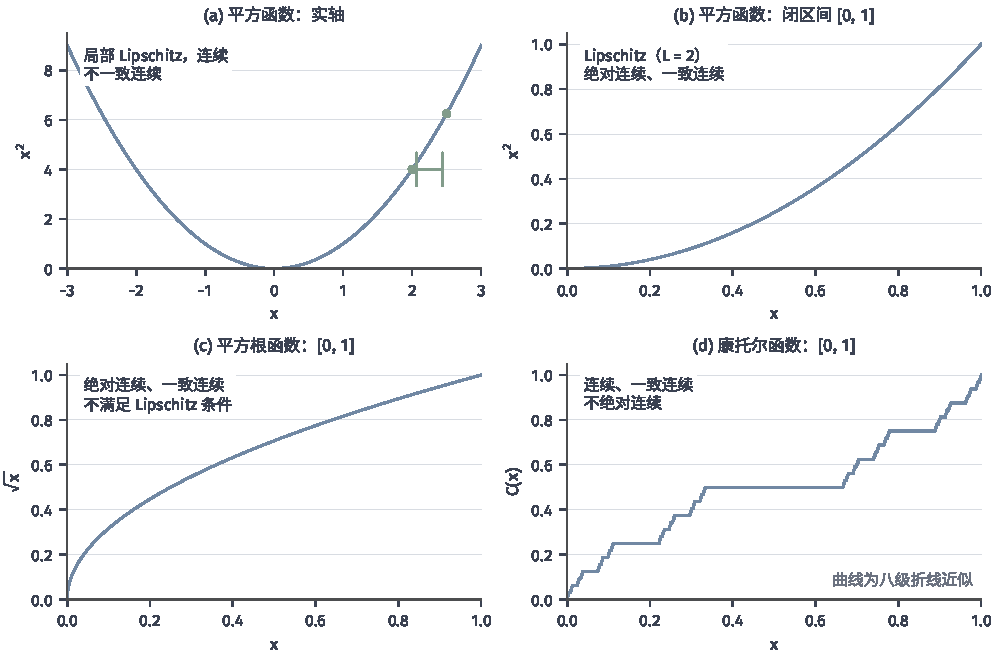
\includegraphics[width=169mm]{figures/01-mathematical-preliminaries-upper/01-mathematical-language-combinatorics-analysis-optimization/matplotlib/continuity-conditions/figure.pdf}
 \caption{连续性条件依赖于函数和定义域。(a)平方函数在实轴上连续且局部Lipschitz，但不一致连续；只展示$[-3,3]$内的曲线，标记对应$x_2=2$、$y_2=2+1/2$，完整反例使用$x_n=n$、$y_n=n+1/n$两列输入。(b)同一函数限制到$[0,1]$后为Lipschitz函数，因而绝对连续且一致连续。(c)$\sqrt x$在$[0,1]$上绝对连续、一致连续，却不是Lipschitz函数。(d)康托尔函数在$[0,1]$上连续且一致连续，但不绝对连续。右下曲线为八级折线近似，性质标注属于极限函数；每条有限折线本身都是Lipschitz函数，图形不能代替不绝对连续的证明。}
 \label{fig:analysis-continuity-conditions}
\end{figure*}

\subsection{闭区间上连续函数的性质}

\subsubsection{有界性与最值}
第~\ref{chap:sets-functions-and-proofs}章已经看到，函数的下确界未必能取到，例如$x$在$(0,1)$上没有最小值。所以在寻找最小值之前，需要先知道什么条件保证最值存在。
关键仍是收敛子列：在闭且有界的集合中，Bolzano--Weierstrass定理~\ref{thm:analysis-bounded-subsequence}给出每个序列的收敛子列，
闭集的序列判据（引理~\ref{lem:analysis-closed-sequence-criterion}）保证极限仍在集合内。
再结合连续性，就能证明函数有界并达到最值。
\begin{theorem}[闭有界集上的极值定理]
\label{thm:analysis-extreme-value}
设$K\subseteq\mathbb R$非空、闭且有界，$f:K\to\mathbb R$连续，则$f$有界，且在$K$上达到最小值和最大值。特别地，结论适用于非空闭区间。
\end{theorem}
\begin{proof}
先证有界。若$f$无界，可选$x_n\in K$使$|f(x_n)|>n$。$K$有界，序列$(x_n)$有收敛子列$x_{n_k}\to x$，闭性保证$x\in K$；连续性给出$f(x_{n_k})\to f(x)$。收敛数列有界，这与$|f(x_{n_k})|>n_k\to\infty$矛盾。

再证达到最小值。$f$有界且$K$非空，所以$m=\inf_K f$是有限实数。对每个$n$选$x_n\in K$使$m\leq f(x_n)<m+1/n$。取收敛子列$x_{n_k}\to x^\star\in K$，连续性给出$f(x_{n_k})\to f(x^\star)$；而$f(x_{n_k})$夹在$m$与$m+1/n_k$之间，也趋于$m$，所以$f(x^\star)=m$。对$-f$重复论证即得最大值。
\end{proof}
定理要求定义域闭、定义域有界且函数连续，三个条件缺一不可。下面三个函数各缺少其中一个条件，下确界都取不到。
\begin{example}[极值定理的条件]
\label{ex:analysis-extrema-failures}
定义域不闭：在$(0,1)$上，连续函数$f(x)=x$的下确界为$0$，但$0$不在定义域中，最小值不存在。

定义域无界：实轴闭但无界。$e^x$在$\mathbb R$上连续，$x\to-\infty$时趋于$0$，下确界为$0$；由于$e^x>0$，下确界取不到。

函数不连续：在$[0,1]$上令$f(0)=1$，$x>0$时$f(x)=x$。定义域闭且有界，但$x\downarrow0$时$f(x)\to0\neq f(0)$，$f$在$0$处不连续。下确界仍为$0$，而$f(0)=1$，$x>0$时$f(x)=x>0$，所以最小值不存在。
\end{example}
三个条件分别排除了一种失效方式：有界性保证序列有收敛子列，闭性保证子列的极限仍在定义域内，连续性保证函数值随子列收敛到极限点处的值。

\subsubsection{介值定理}
闭区间上的连续函数还有另一条性质：函数从一个端点值变到另一个端点值时，取遍二者之间的每个数值。
这一结论要求两个端点之间的整段都属于定义域，比极值定理的“闭且有界”更具体。
\begin{theorem}[闭区间上的介值定理]
\label{thm:analysis-intermediate-value}
设$a,b\in\mathbb R$、$a<b$，$f:[a,b]\to\mathbb R$连续。则
\[
 \begin{gathered}
 \forall c\in[\min\{f(a),f(b)\},\max\{f(a),f(b)\}],\\
 \exists\xi\in[a,b],\quad f(\xi)=c.
 \end{gathered}
\]
若$\min\{f(a),f(b)\}<c<\max\{f(a),f(b)\}$，则可取$\xi\in(a,b)$。
\end{theorem}
\begin{proof}
$c=f(a)$或$c=f(b)$时，直接取相应端点。下面设$f(a)<c<f(b)$，令
$S=\{x\in[a,b]:f(x)\leq c\}$。因为$a\in S$且$S$有上界$b$，实数的确界性质给出$u=\sup S\in[a,b]$。
对每个正整数$n$，可选$x_n\in S$满足$u-1/n<x_n\leq u$，于是$x_n\to u$。
连续性使$f(x_n)\to f(u)$，由$f(x_n)\leq c$得到$f(u)\leq c$；又因$f(b)>c$，所以$u\neq b$。
若$f(u)<c$，连续性保证$u$右侧充分近的点仍有函数值小于$c$；
由于$u<b$，可在$[a,b]$内选到这样的点$v>u$。于是$v\in S$，与$u$是$S$的上界矛盾。
因此$f(u)=c$。又因$f(a)<c$，有$u\neq a$，所以$u\in(a,b)$。
若$f(a)>c>f(b)$，对$-f$与$-c$应用同一论证即可。
\end{proof}
定理用到了两个端点之间的整段都属于定义域。定义域闭且有界但有缺口时，介值性可能失效。
\begin{example}[有缺口的定义域上不取中间值]
\label{ex:analysis-intermediate-value-gap}
令$X=[-2,-1]\cup[1,2]$，在$[-2,-1]$上取$f(x)=0$，在$[1,2]$上取$f(x)=1$。对每个$a\in X$取$\delta=1$：若$x\in X$且$|x-a|<1$，则$x$与$a$属于同一段，$f(x)=f(a)$。所以$f$在$X$上连续。$X$闭且有界，$f$在$-2$与$2$处分别取$0$和$1$，却不取中间值$1/2$。
\end{example}
极值定理在这个定义域上仍然成立；闭且有界足以保证最值，却不能代替介值定理中的区间条件。

\par\Needspace{10\baselineskip}
\section{微分的定义}
\label{sec:analysis-derivatives-linear-approximation}

连续性只说明输入接近时函数值也接近，没有说明函数值随输入变化的快慢。本节先用差商的极限定义导数，再把导数改写为函数增量的一阶线性近似，由此定义微分。

\subsection{导数}

\paragraph{差商}
设$f$在包含$a$的某个开区间内有定义。输入从$a$变为$a+h$时，函数增量为$\Delta f=f(a+h)-f(a)$。当$h\neq0$时，比值$\Delta f/h$称为差商，表示这两个输入之间的平均变化率；在图形上，它是连接$(a,f(a))$与$(a+h,f(a+h))$两点的割线斜率。

\paragraph{导数}
让$h$趋于零，两点之间的平均变化率就收缩为一点处的变化率。若差商在$h\to0$时趋于一个有限实数，就定义
\[
 f'(a)=\lim_{h\to0}\frac{f(a+h)-f(a)}h,
\]
称其为$f$在$a$处的\term{导数}（derivative），并称$f$在$a$处可导。导数给出该点的瞬时变化率，在图形上是该点切线的斜率。

若$f$在某个区间内每点都可导，则$a\mapsto f'(a)$又构成一个函数，称为导函数。例如$f(x)=x^2$时，差商$[(a+h)^2-a^2]/h=2a+h$，令$h\to0$得$f'(a)=2a$。

\paragraph{单侧导数}
在区间端点处，或在左右两侧变化方式不同的点处，需要分别考察两侧的差商。
只让$h>0$或只让$h<0$取极限，分别得到右导数$f'_+(a)$和左导数$f'_-(a)$。在内点处，双侧导数存在，当且仅当左右导数都存在、有限且相等。在闭区间端点讨论导数时，本章明确采用从区间内部取得的单侧导数；未特别说明时，内点处的导数都指有限的双侧导数。

\subsection{可微函数}

导数还可以写成函数增量的近似形式。差商趋于$f'(a)$，等价于$f(a+h)-f(a)-f'(a)h$除以$h$后趋于零，即
\begin{equation}
 f(a+h)=f(a)+f'(a)h+o(|h|),\qquad h\to0,
\label{eq:analysis-scalar-first-order}
\end{equation}
其中$o(|h|)$表示除以$|h|$后趋于零的量，沿用第~\ref{sec:comb-growth-scales}节的记号。

式~\eqref{eq:analysis-scalar-first-order}把函数增量分成线性部分$f'(a)h$与高阶余项。反过来，也可以不先假定导数存在，只要求增量有这样的分解：若存在实数$A$，使$h\to0$时$f(a+h)-f(a)=Ah+o(|h|)$，就称$f$在$a$处\term{可微}（differentiable）。两边除以$h$再令$h\to0$，可知差商趋于$A$，所以$f$在$a$处可导且$A=f'(a)$。结合式~\eqref{eq:analysis-scalar-first-order}，一元实函数在内点处可导与可微等价。

可微的分解中，线性部分把输入增量$h$映成函数增量的一阶预测值。线性映射$h\mapsto f'(a)h$称为$f$在$a$处的\term{微分}（differential），记为$\mathrm df_a(h)$。导数$f'(a)$是一个实数，微分则是以它为系数的线性映射。常用记号$\mathrm df=f'(x)\,\mathrm dx$表达同一关系，其中$\mathrm dx$表示输入增量。实际的有限增量$\Delta f$还包含余项，一般不等于微分。

微分与实际增量之差就是式~\eqref{eq:analysis-scalar-first-order}中的余项。用具体数值比较二者，可以看到余项有多大。
\begin{example}[平方函数在$a=3$处的微分]
\label{ex:analysis-square-differential}
设$f(x)=x^2$，$a=3$，则$f'(3)=6$，微分为$\mathrm df_3(h)=6h$。取$h=0.1$，微分给出$0.6$，实际增量为$3.1^2-3^2=0.61$。一般地，
\[
 (3+h)^2-3^2-6h=h^2,
\]
所以两者之差恰为$h^2$，$h=0.1$时为$0.01$。余项$h^2$除以$|h|$后趋于零，符合式~\eqref{eq:analysis-scalar-first-order}。
\end{example}
\begin{example}[$x^3-3x$在$a=1/2$处的一阶近似]
\label{ex:analysis-cubic-linear-approximation}
设$f(x)=x^3-3x$。由$(a+h)^3=a^3+3a^2h+3ah^2+h^3$，差商为$3a^2-3+3ah+h^2$，令$h\to0$得$f'(a)=3a^2-3$。取$a=1/2$，则$f(1/2)=-11/8$、$f'(1/2)=-9/4$，一阶近似为
\begin{equation}
 T_1(\tfrac12+h)=-\frac{11}{8}-\frac94h.
\label{eq:analysis-cubic-linear-model}
\end{equation}
取$h=0.1$，$T_1(0.6)=-1.600$，而$f(0.6)=0.216-1.8=-1.584$，近似值比真值小$0.016$。
\end{example}
第一例的余项恰为$h^2$；第二例余下的$0.016$来自函数图像的弯曲，第~\ref{sec:analysis-second-order-curvature}节将用二阶导数解释它。

可微还蕴含连续。若$f$在$a$处可微，由式~\eqref{eq:analysis-scalar-first-order}，$h\to0$时$f(a+h)-f(a)=f'(a)h+o(|h|)\to0$，即$f$在$a$处连续。

连续却只是可微的必要条件，并不充分。
\begin{example}[绝对值函数在原点连续而不可微]
\label{ex:analysis-absolute-value-not-differentiable}
设$f(x)=|x|$。由$\bigl||x|-|a|\bigr|\leq|x-a|$，$f$在每一点连续。在原点，差商为$|h|/h$：$h>0$时等于$1$，$h<0$时等于$-1$。所以$f'_+(0)=1$、$f'_-(0)=-1$，左右导数不相等，$f$在$0$处不可导，也就不可微。
\end{example}
阶跃函数在原点不连续，由上述必要条件，它在原点也不可微。图~\ref{fig:analysis-continuity-counterexamples}比较了连续且可微、连续但不可微与不连续三种情形。
\begin{figure*}[htbp]
 \centering
 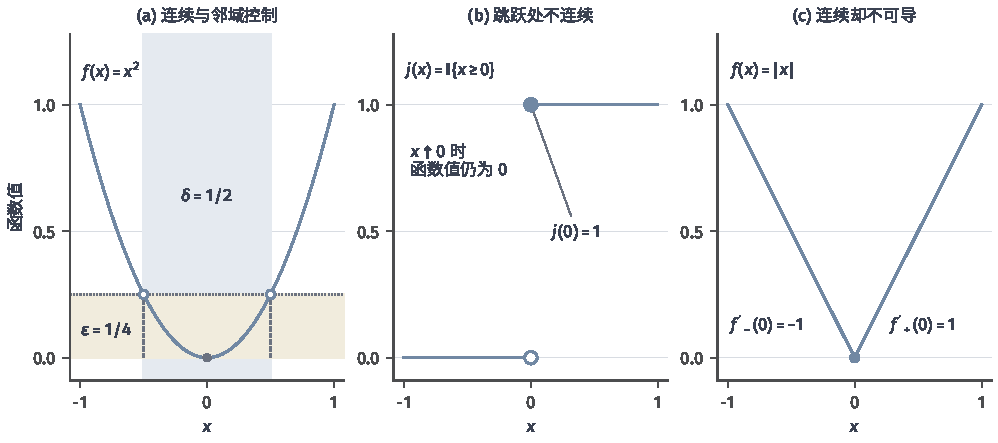
\includegraphics[width=169.0mm]{figures/01-mathematical-preliminaries-upper/01-mathematical-language-combinatorics-analysis-optimization/matplotlib/analysis-continuity-counterexamples/figure.pdf}
 \caption{平方函数、绝对值函数与阶跃函数在原点的差别。平方函数连续且可微；绝对值函数连续，但左右导数不同；阶跃函数的左右极限不同。连续性控制函数值的极限，可微性还要求差商具有同一个有限极限。}
 \label{fig:analysis-continuity-counterexamples}
\end{figure*}

\subsection{连续可微函数}

可导只要求每一点的差商各自有极限，并不要求邻近位置的导数接近该点的导数。
若进一步要求导函数本身连续，就得到更强的条件：若$f$在开区间$I$上可导且$f'$在$I$上连续，就称$f$连续可微，记为$f\in C^1(I)$。

在闭区间上使用$C^1([a,b])$时，要求$f$在$[a,b]$上连续、在$(a,b)$内可导，且$f'$能连续延拓到两个端点。由后文的Lagrange中值定理（定理~\ref{thm:analysis-lagrange-mean-value}）可以证明，延拓值就是相应的单侧导数。

处处可导与连续可微确实不同：导函数可能在某点不连续。
\begin{example}[处处可导而导函数不连续]
\label{ex:analysis-derivative-not-continuous}
令$f(0)=0$，$x\neq0$时$f(x)=x^2\sin(1/x)$。在原点，差商为$h\sin(1/h)$；由$|h\sin(1/h)|\leq|h|$及夹逼定理，它趋于$0$，所以$f'(0)=0$。在非零点，
\[
 f'(x)=2x\sin\frac1x-\cos\frac1x,
\]
这一公式将在示例~\ref{ex:analysis-oscillating-derivative-formula}中由求导规则得到。取$x_n=1/(2\pi n)$，则$x_n\to0$，而$\sin(1/x_n)=0$、$\cos(1/x_n)=1$，故$f'(x_n)=-1$。$f'(x_n)$不趋于$f'(0)=0$，所以$f'$在$0$处不连续：$f$在$\mathbb R$上处处可导，却不属于$C^1(\mathbb R)$。
\end{example}
导数在原点附近的振荡来自$-\cos(1/x)$一项，它在$-1$与$1$之间反复取值。因此$C^1$是比处处可导更强的条件。

\section{微分的运算法则}
\label{sec:analysis-scalar-chain-rules}

本节由已知函数的导数求组合函数的导数。以下设$f,g$在所讨论的点$a$的某个开邻域内有定义，并在$a$处可导；各条规则都由差商的极限或式~\eqref{eq:analysis-scalar-first-order}的一阶展开得到。

\subsection{四则运算的求导}

\paragraph{和与数乘}
和的差商等于两个差商之和，常数倍的差商等于差商的同一常数倍。令$h\to0$，由极限的和与数乘法则得到$(f+g)'(a)=f'(a)+g'(a)$与$(cf)'(a)=cf'(a)$，其中$c$为实常数。差$f-g=f+(-1)g$的导数由这两条合并得到。

\paragraph{乘积法则}
乘积的增量可以拆成三部分。记$\Delta f=f(a+h)-f(a)$、$\Delta g=g(a+h)-g(a)$，则
\[
 f(a+h)g(a+h)-f(a)g(a)=g(a)\,\Delta f+f(a)\,\Delta g+\Delta f\,\Delta g.
\]
由式~\eqref{eq:analysis-scalar-first-order}，前两项之和为$[f'(a)g(a)+f(a)g'(a)]h+o(|h|)$；两个增量都是$O(|h|)$，它们的乘积属于$O(h^2)$，也是$o(|h|)$。所以$fg$在$a$处可微，一次项的系数就是导数。连同上一段的和法则，得到
\begin{equation}
 \begin{aligned}
 (f+g)'(a)&=f'(a)+g'(a),\\
 (fg)'(a)&=f'(a)g(a)+f(a)g'(a).
 \end{aligned}
\label{eq:analysis-scalar-sum-product-rules}
\end{equation}

\paragraph{商法则}
设$g(a)\neq0$。可导蕴含连续，按商的连续性中的论证，$g$在$a$附近不为零，$f/g$在$a$附近有定义。先求倒数的导数：
\[
 \frac1h\Bigl(\frac1{g(a+h)}-\frac1{g(a)}\Bigr)
 =-\frac{g(a+h)-g(a)}h\cdot\frac1{g(a+h)g(a)}
 \longrightarrow-\frac{g'(a)}{g(a)^2},
\]
其中用到$g(a+h)\to g(a)$。再把$f/g$写成$f\cdot(1/g)$并使用乘积法则，得到
\[
 \left(\frac fg\right)'(a)
 =\frac{f'(a)}{g(a)}-\frac{f(a)g'(a)}{g(a)^2}
 =\frac{f'(a)g(a)-f(a)g'(a)}{g(a)^2}.
\]
条件$g(a)\neq0$既保证$f/g$在$a$附近有定义，也保证公式右侧有意义。

\subsection{复合函数求导}

复合函数的输入变化先经过内层，再传入外层；总的一阶变化由两层的局部变化率共同决定。
若$f$在$a$处可导，$g$在$f(a)$处可导，且$g\circ f$在$a$附近有定义，则
\begin{equation}
 (g\circ f)'(a)=g'(f(a))f'(a).
\label{eq:analysis-scalar-chain-rule}
\end{equation}
这称为\term{链式法则}（chain rule）。

证明时，记$b=f(a)$、$k(h)=f(a+h)-f(a)$。由$f$的一阶展开，$k(h)=f'(a)h+o(|h|)$，所以$k(h)\to0$，并且充分小的$h$满足$|k(h)|\leq(|f'(a)|+1)|h|$。把$g$在$b$处的一阶展开写成
\[
 g(b+k)=g(b)+g'(b)k+|k|\,\varepsilon(k),
\]
其中$k\neq0$时$\varepsilon(k)=[g(b+k)-g(b)-g'(b)k]/|k|$，它在$k\to0$时趋于零，并规定$\varepsilon(0)=0$。代入$k=k(h)$，得到
\[
 g(f(a+h))-g(f(a))=g'(b)f'(a)h+g'(b)\,o(|h|)+|k(h)|\,\varepsilon(k(h)).
\]
最后一项的绝对值不超过$(|f'(a)|+1)|h|\,|\varepsilon(k(h))|$，而$\varepsilon(k(h))\to0$，所以它也是$o(|h|)$。于是$g\circ f$在$a$处可微，一次项系数为$g'(f(a))f'(a)$。规定$\varepsilon(0)=0$使上式在$k(h)=0$时同样成立，所以证明也覆盖$f'(a)=0$等中间增量可能为零的情形，无需除以$k(h)$。

\subsection{反函数求导}
第~\ref{sec:analysis-inverse-continuity}节已经证明，区间上连续且严格单调的函数有连续的反函数。现在判断反函数何时可导，以及它的导数怎样由原函数的导数决定。

设$f:I\to J$在区间$I$上连续且严格单调，$J=f(I)$，其反函数为$g=f^{-1}$。设$a$是$I$的内点，$f$在$a$处可导且$f'(a)\neq0$，记$b=f(a)$。取$r>0$使$a-r,a+r\in I$；由介值定理，$J$包含$f(a-r)$与$f(a+r)$之间的整段，而$b$严格位于二者之间，所以$b$是$J$的内点。对充分小的$k\neq0$，令$h=g(b+k)-a$。$g$是一一对应，所以$h\neq0$；$g$连续，所以$k\to0$时$h\to0$。由$f(a+h)=b+k$，
\[
 \frac{g(b+k)-g(b)}k
 =\frac{h}{f(a+h)-f(a)}\longrightarrow\frac1{f'(a)}.
\]
因此$g$在$b$处可导，且$g'(b)=1/f'(a)$。

对恒等式$f(g(y))=y$使用链式法则，也会得到同一公式；但链式法则要求$g$已经可导，所以上面先用差商证明可导性。公式需要两个条件：$f$在所讨论的区间上一一对应，且在对应点处$f'(a)\neq0$。例如$x^3$在$0$处导数为零，其反函数$\sqrt[3]y$在$0$处的差商为$1/(\sqrt[3]k)^2$，$k\to0$时无界，所以反函数在$0$处不可导。

\subsection{基本初等函数的导数}
\label{sec:analysis-elementary-derivatives}

有了四则运算、复合与反函数的求导规则，复杂函数的求导就归结为少数基本函数的导数。以下逐类从差商推出这些导数，并注明成立范围。

\subsubsection{常数函数与整数幂函数}
常数函数$f(x)=c$的差商恒为零，恒等函数$f(x)=x$的差商恒为$1$，所以二者的导数分别为$0$和$1$。
对正整数$m$，把$x^m$看成$m$个恒等函数的乘积，反复使用乘积法则：每一项只对一个因子求导、保留其余$m-1$个因子，共有$m$项，每项都等于$x^{m-1}$，所以$(x^m)'=mx^{m-1}$。
$m=0$时$x^0=1$是常数函数，公式右侧按$0$理解。

对负整数$m=-n$（$n$为正整数），在$x\neq0$处把$x^m$写成$1/x^n$，由商法则，
\[
 \Bigl(\frac1{x^n}\Bigr)'=-\frac{nx^{n-1}}{x^{2n}}=-nx^{-n-1}=mx^{m-1},
\]
仍是同一形式。于是
\[
 \begin{aligned}
 (c)'&=0,\\
 (x^m)'&=mx^{m-1}\qquad(m\in\mathbb Z),
 \end{aligned}
\]
其中$m\geq0$时对全体实数$x$成立，$m<0$时要求$x\neq0$。

\subsubsection{正弦函数与余弦函数}
三角函数采用弧度制。第~\ref{sec:analysis-function-limits}节已经得到$\sin h/h\to1$与$(\cos h-1)/h\to0$。由正弦、余弦的加法公式，两个差商都能写成这两个比值的组合：
\[
 \begin{aligned}
 \frac{\sin(x+h)-\sin x}{h}
 &=\sin x\frac{\cos h-1}{h}+\cos x\frac{\sin h}{h}
 \longrightarrow\cos x,\\
 \frac{\cos(x+h)-\cos x}{h}
 &=\cos x\frac{\cos h-1}{h}-\sin x\frac{\sin h}{h}
 \longrightarrow-\sin x.
 \end{aligned}
\]
因此
\[
 \begin{aligned}
 (\sin x)'&=\cos x,\\
 (\cos x)'&=-\sin x,
 \end{aligned}
\]
两式对全体实数$x$成立。
若改用角度制，基本极限$\sin h/h$会多出比例系数$\pi/180$，导数公式也随之多出这个系数。

\subsubsection{指数函数}
自然指数函数满足$e^{x+h}=e^xe^h$。由第~\ref{sec:analysis-function-limits}节的基本极限$(e^h-1)/h\to1$，得到
\[
 \frac{e^{x+h}-e^x}{h}=e^x\frac{e^h-1}{h}\longrightarrow e^x.
\]
推导只用到由级数得到的乘法公式和这个基本极限，不依赖其他求导结果。因此
\[
 (e^x)'=e^x\qquad(x\in\mathbb R).
\]

\subsubsection{对数函数与实数幂函数}
自然对数定义为指数函数的反函数，先要确认这个反函数存在。$e^x$连续、严格递增且恒为正，$x\to-\infty$时趋于$0$，$x\to+\infty$时趋于$+\infty$。对任意$y>0$，先选两点使指数值分别小于和大于$y$，再用介值定理得到原像；严格递增保证原像唯一。所以指数函数是$\mathbb R$到$(0,\infty)$的一一对应，其反函数称为自然对数，记为$\log x$（也记$\ln x$），定义在$x>0$上。指数函数的导数$e^x$处处非零，由反函数求导，$(\log x)'=1/e^{\log x}=1/x$。

设$a>0$且$a\neq1$。实数次幂定义为$a^x=e^{x\log a}$，它的反函数$\log_a x$等于$(\log x)/(\log a)$，因为$a^{(\log x)/(\log a)}=e^{\log x}=x$。由链式法则，$(a^x)'=e^{x\log a}\log a=a^x\log a$；由数乘法则，$(\log_a x)'=1/(x\log a)$。
对任意实数$\alpha$，在$x>0$上定义$x^\alpha=e^{\alpha\log x}$，链式法则给出$(x^\alpha)'=e^{\alpha\log x}\cdot\alpha/x=\alpha x^{\alpha-1}$。于是
\[
 \begin{aligned}
 (\log x)'&=\frac1x, &&x>0,\\
 (\log_a x)'&=\frac1{x\log a}, &&x>0,\\
 (x^\alpha)'&=\alpha x^{\alpha-1}, &&x>0,\\
 (a^x)'&=a^x\log a, &&x\in\mathbb R.
 \end{aligned}
\]
这里没有为负数底数定义任意实数次幂，所以$x^\alpha$的公式只在$x>0$上使用。

\subsubsection{基本初等函数导数表}
表~\ref{tab:analysis-elementary-derivatives}汇总了上面得到的公式及成立范围。
把它们与四则运算法则、链式法则和反函数求导结合，就能求出由这些函数经有限次运算与复合得到的初等函数的导数。
示例~\ref{ex:analysis-derivative-not-continuous}在非零点使用的导数公式，就可以这样由乘积法则、链式法则和正弦导数得到。
\begin{example}[$x^2\sin(1/x)$在非零点的导数]
\label{ex:analysis-oscillating-derivative-formula}
设$x\neq0$。内层函数$1/x=x^{-1}$的导数为$-1/x^2$，由链式法则和正弦导数，$\bigl(\sin(1/x)\bigr)'=-\cos(1/x)/x^2$。再由乘积法则，
\[
 \Bigl(x^2\sin\frac1x\Bigr)'
 =2x\sin\frac1x+x^2\Bigl(-\frac1{x^2}\cos\frac1x\Bigr)
 =2x\sin\frac1x-\cos\frac1x.
\]
\end{example}
这些规则不能用于原点，因为$\sin(1/x)$在$0$处没有定义；原点处的导数须直接用差商计算，正如示例~\ref{ex:analysis-derivative-not-continuous}所做。
\begin{table}[htbp]
 \centering\small
 \begin{tabular}{@{}lll@{}}
 \toprule
 函数 & 导数 & 成立范围\\
 \midrule
 $c$ & $0$ & $x\in\mathbb R$\\
 $x^m$（$m\in\mathbb Z$） & $mx^{m-1}$ & $m\geq0$时$x\in\mathbb R$；$m<0$时$x\neq0$\\
 $x^\alpha$（$\alpha\in\mathbb R$） & $\alpha x^{\alpha-1}$ & $x>0$\\
 $\sin x$ & $\cos x$ & $x\in\mathbb R$\\
 $\cos x$ & $-\sin x$ & $x\in\mathbb R$\\
 $e^x$ & $e^x$ & $x\in\mathbb R$\\
 $a^x$（$a>0$，$a\neq1$） & $a^x\log a$ & $x\in\mathbb R$\\
 $\log x$ & $1/x$ & $x>0$\\
 $\log_a x$（$a>0$，$a\neq1$） & $1/(x\log a)$ & $x>0$\\
 \bottomrule
 \end{tabular}
 \caption{基本初等函数的导数。三角函数采用弧度制，$\log$为自然对数。}
 \label{tab:analysis-elementary-derivatives}
\end{table}

\section{闭区间上可微函数的性质}

导数记录一点处的变化率。本节把它与区间上的极值、端点之间的净变化以及两点之间的变化幅度联系起来。
涉及闭区间$[a,b]$的中值结论都只要求函数在$[a,b]$上连续、在$(a,b)$内可导，不要求端点处的单侧导数存在。

\subsection{局部极值与驻点}

\paragraph{局部极值}
导数只反映一点附近的变化，与它对应的是只比较邻近函数值的极值，而不是整个定义域上的最值。
设$c$属于$f$的定义域。若存在$r>0$，使定义域中所有满足$|x-c|<r$的$x$都有$f(x)\geq f(c)$，则称$c$为$f$的局部极小点；若其中$x\neq c$的点都满足严格不等式$f(x)>f(c)$，则称$c$为严格局部极小点。
把不等号反向，就得到局部极大点和严格局部极大点。

\paragraph{Fermat定理}
局部极值比较的是邻近的函数值，导数是差商的极限。在内点处可以从两侧取差商，差商的符号把这两种信息联系起来。
\begin{theorem}[Fermat定理]
\label{thm:analysis-fermat}
设$a<b$，$f:[a,b]\to\mathbb R$，$c\in(a,b)$。若$f$在$c$处可导，且$c$为$f$的局部极小点或局部极大点，则
\begin{equation}
 f'(c)=0.
\label{eq:analysis-scalar-first-order-necessary}
\end{equation}
\end{theorem}
\begin{proof}
设$c$为局部极小点。充分小的$h\neq0$满足$f(c+h)-f(c)\geq0$，
故$h>0$时差商非负，$h<0$时差商非正。
两侧差商趋于同一个有限导数，因而同时有$f'(c)\geq0$与$f'(c)\leq0$，即$f'(c)=0$。
局部极大点对$-f$应用同一论证即可。
\end{proof}
导数为零的点称为\term{驻点}（stationary point）。Fermat定理说明，内点处可导的局部极值点必为驻点。这一必要条件既不能逆用，也不能搬到端点上。
\begin{example}[非极值的驻点与端点处的极值]
\label{ex:analysis-fermat-condition-failures}
设$f(x)=x^3$。由$(x^3)'=3x^2$，$f'(0)=0$，所以$0$是驻点。但$x<0$时$f(x)<0=f(0)$，$x>0$时$f(x)>0=f(0)$；$0$的任何邻域内都有比$f(0)$更小和更大的函数值，所以$0$不是局部极值点。

再设$g(x)=x$，$x\in[0,1]$。$g$在端点$0$处取最小值，但右导数$g'_+(0)=1\neq0$。端点处只能从一侧取差商，Fermat定理证明中两侧差商的符号对比无法进行。
\end{example}
因此Fermat定理只给出内点处极值的必要条件。驻点是否为极值点，还要看函数在它两侧的增减；第~\ref{sec:analysis-monotonicity}节将用导数的符号判断这一点。

\subsection{中值定理}

\subsubsection{Rolle定理}
若函数在区间两端取同一值，整段的净变化为零。
在连续、可导的条件下，区间内部必有一点的瞬时变化率也为零。
\begin{theorem}[Rolle定理]
\label{thm:analysis-rolle}
设$a<b$，$f:[a,b]\to\mathbb R$在$[a,b]$上连续、在$(a,b)$内可导。
若$f(a)=f(b)$，则
\[
 \exists c\in(a,b),\qquad f'(c)=0.
\]
\end{theorem}
\begin{proof}
若$f$恒定，任取$c\in(a,b)$即可。
否则存在$x_0\in(a,b)$使$f(x_0)\neq f(a)$。
由闭区间上的极值定理~\ref{thm:analysis-extreme-value}，$f$在$[a,b]$上达到最大值和最小值。若$f(x_0)>f(a)=f(b)$，最大值不小于$f(x_0)$，严格大于两端的值，所以最大值必在某个内点达到；
若$f(x_0)<f(a)=f(b)$，同理最小值必在某个内点达到。
这个内点是局部极值点，$f$在那里可导，由Fermat定理~\ref{thm:analysis-fermat}，导数为零。
\end{proof}

\subsubsection{Lagrange中值定理}
两端取值不同时，可以先减去连接两个端点的直线，使剩余函数在两端相等，再对它应用Rolle定理。
这样就把整段的平均变化率与某个内点的瞬时变化率联系起来。
\begin{theorem}[Lagrange中值定理]
\label{thm:analysis-lagrange-mean-value}
设$a<b$，$f:[a,b]\to\mathbb R$在$[a,b]$上连续、在$(a,b)$内可导，则存在$c\in(a,b)$使
\begin{equation}
 f(b)-f(a)=f'(c)(b-a).
\label{eq:analysis-mean-value-theorem}
\end{equation}
等价地，$f'(c)=[f(b)-f(a)]/(b-a)$。
\end{theorem}
\begin{proof}
令
\[
 H(x)=f(x)-f(a)-\frac{f(b)-f(a)}{b-a}(x-a).
\]
$H$在$[a,b]$上连续、在$(a,b)$内可导，并满足$H(a)=H(b)=0$。
Rolle定理给出某个$c\in(a,b)$使
$H'(c)=f'(c)-[f(b)-f(a)]/(b-a)=0$，整理即得结论。
\end{proof}
这就是Lagrange\term{中值定理}（mean value theorem）的含义：区间上的平均变化率等于某个内点处的瞬时变化率。
定理只要求函数在每个内点可导，不要求导函数连续。

图~\ref{fig:analysis-process-mean-value-parallel}以$f(x)=x^2$、区间$[0,1]$为例：端点割线的斜率为$1$，$c=1/2$处的切线斜率$f'(1/2)=1$与之相等，两线平行。
\begin{figure}[!htbp]
 \centering
 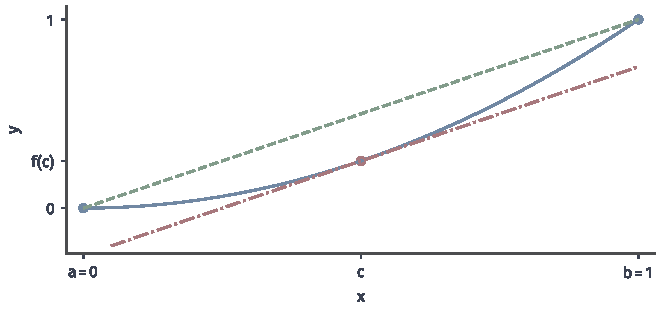
\includegraphics[width=112.0mm]{figures/01-mathematical-preliminaries-upper/01-mathematical-language-combinatorics-analysis-optimization/matplotlib/chapter3-concept-processes/mean-value-parallel.pdf}
 \caption{$f(x)=x^2$在$[0,1]$上，绿虚线为端点割线，红点划线为$c=1/2$处的切线。两线平行，因为$f'(c)=1=[f(1)-f(0)]/(1-0)$。两线高度不同：相等的是斜率，两条直线并不重合。}
 \label{fig:analysis-process-mean-value-parallel}
\end{figure}

\subsubsection{Cauchy中值定理}
比较两个函数在同一区间上的变化时，可以把两者的端点增量放进同一个辅助函数，再应用Rolle定理。
结论先写成交叉相乘的形式，这样不需要假设任何分母非零。
\begin{theorem}[Cauchy中值定理]
\label{thm:analysis-cauchy-mean-value}
设$a<b$，$f,g:[a,b]\to\mathbb R$均在$[a,b]$上连续、在$(a,b)$内可导，则存在$c\in(a,b)$使
\[
 (f(b)-f(a))g'(c)=(g(b)-g(a))f'(c).
\]
若进一步有$g'(x)\neq0$对每个$x\in(a,b)$成立，则$g(b)\neq g(a)$，并可写为
\[
 \frac{f(b)-f(a)}{g(b)-g(a)}=\frac{f'(c)}{g'(c)}.
\]
\end{theorem}
\begin{proof}
令
\[
 \begin{aligned}
 H(x)={}&(f(b)-f(a))(g(x)-g(a))\\
        &-(g(b)-g(a))(f(x)-f(a)).
 \end{aligned}
\]
$H$继承两函数的连续、可导条件，并有$H(a)=H(b)=0$。
应用Rolle定理得$H'(c)=0$，展开导数即为交叉相乘形式。
若$g'$在$(a,b)$内处处非零，$g(b)=g(a)$会使Rolle定理给出某个内点处$g'=0$，产生矛盾，故$g(b)\neq g(a)$。
此时$g'(c)\neq0$，交叉相乘形式两边同除以$(g(b)-g(a))g'(c)$，即得比值形式。
\end{proof}
取$g(x)=x$，则$g'=1$，比值形式就是Lagrange中值定理。

\subsection{单调性}
\label{sec:analysis-monotonicity}

\subsubsection{导数符号与单调性}
中值定理把任意两点之间的函数增量写成某个内点处的导数乘以输入增量，所以导数的符号可以控制整段的增减。
这里的关键是任意两点之间的整段都属于定义域。
\begin{theorem}[导数符号与单调性]
\label{thm:analysis-derivative-monotonicity}
设$a<b$，$f:[a,b]\to\mathbb R$在$[a,b]$上连续、在$(a,b)$内可导。
若$f'(x)\geq0$对所有$x\in(a,b)$成立，则$f$在$[a,b]$上单调不减；若处处有$f'(x)>0$，则严格递增。
相应地，$f'\leq0$蕴含单调不增，$f'<0$蕴含严格递减。
若$f'$在$(a,b)$内恒为零，则$f$在$[a,b]$上为常数。
\end{theorem}
\begin{proof}
任取$a\leq x<y\leq b$，在$[x,y]$上应用Lagrange中值定理，存在$\xi\in(x,y)$使
\[
 f(y)-f(x)=f'(\xi)(y-x).
\]
因为$y-x>0$，右侧的符号由$f'(\xi)$决定，于是得到四种单调性结论。
导数恒为零时，任意两点的函数值都相等，所以函数为常数。
\end{proof}
导数恒为零只保证函数在每个区间上为常数。若定义域由分离的区间组成，各段的常数未必相同：例如在$(0,1)\cup(2,3)$上，左段取$0$、右段取$1$的函数导数处处为零，却不是常数。中值定理不能跨过定义域的缺口使用。

导数为零也不妨碍严格单调：$x^3$在整个实轴上严格递增，因为$x<y$时$y^3-x^3=(y-x)(x^2+xy+y^2)>0$，但它在$0$处导数为零。因此“导数处处严格为正”是严格递增的充分条件，不是必要条件。

\subsubsection{驻点的一阶导数判别}
驻点条件本身不能判定极值，示例~\ref{ex:analysis-fermat-condition-failures}中的$x^3$在驻点$0$两侧都递增。
单调性定理把导数符号转化为增减方向，于是可以比较驻点两侧的变化：先降后升给出极小，先升后降给出极大。
\begin{theorem}[驻点的一阶导数判别]
\label{thm:analysis-first-derivative-test}
设$r>0$，$f$在$[c-r,c+r]$上连续、在$(c-r,c+r)$内可导，且$f'(c)=0$。
若
\[
 f'(x)<0\quad(c-r<x<c),\qquad
 f'(x)>0\quad(c<x<c+r),
\]
则$c$为$f$的严格局部极小点。
若两个区间上的导数符号分别为正和负，则$c$为$f$的严格局部极大点。
\end{theorem}
\begin{proof}
先考虑左负右正的情形。对$c-r<x<c$，$f$在$[x,c]$上连续，且在$(x,c)$内$f'<0$，由定理~\ref{thm:analysis-derivative-monotonicity}，$f$在$[x,c]$上严格递减，故$f(x)>f(c)$；
对$c<x<c+r$，在$[c,x]$上同理得到$f$严格递增，也有$f(x)>f(c)$。
所以$c$两侧充分近的异点都有更大的函数值，$c$为严格局部极小点。
左正右负时反向比较，得到$f(x)<f(c)$，因此$c$为严格局部极大点。
\end{proof}
判别法只需检查导数在驻点两侧的符号。导数能够因式分解时，各因子的符号就给出导数的符号。
\begin{example}[$x^3-3x$的驻点]
\label{ex:analysis-cubic-stationary-points}
设$f(x)=x^3-3x$，则$f'(x)=3x^2-3=3(x-1)(x+1)$，驻点为$x=\pm1$。在定理~\ref{thm:analysis-first-derivative-test}中取$r=1$。

对$x=1$：$0<x<1$时$x-1<0$、$x+1>0$，故$f'(x)<0$；$1<x<2$时两个因子都为正，故$f'(x)>0$。导数由负变正，$1$是严格局部极小点，$f(1)=-2$。

对$x=-1$：$-2<x<-1$时两个因子都为负，故$f'(x)>0$；$-1<x<0$时$x-1<0$、$x+1>0$，故$f'(x)<0$。导数由正变负，$-1$是严格局部极大点，$f(-1)=2$。

$1$只是局部极小点：$x\to-\infty$时$f(x)\to-\infty$，$f$在$\mathbb R$上没有最小值。
\end{example}
若导数在驻点两侧同号，例如$x^3$在$0$两侧都有$f'(x)=3x^2>0$，函数在驻点两侧沿同一方向变化，驻点就不是极值点。

\subsection{Lipschitz条件}

导数的符号控制增减方向；若还能统一限制导数的绝对值，就可以控制任意两点之间的变化幅度。
中值定理把这一导数上界直接转为第~\ref{sec:analysis-continuity-relations}节定义的Lipschitz条件。
\begin{theorem}[有界导数与Lipschitz条件]
\label{thm:analysis-bounded-derivative-lipschitz}
设$a<b$，$f:[a,b]\to\mathbb R$在$[a,b]$上连续、在$(a,b)$内可导。
若存在有限常数$L\geq0$使$|f'(x)|\leq L$对所有$x\in(a,b)$成立，则
\[
 \forall x,y\in[a,b],\qquad |f(y)-f(x)|\leq L|y-x|.
\]
即$f$在$[a,b]$上为Lipschitz连续函数，$L$是一个Lipschitz常数。
\end{theorem}
\begin{proof}
$x=y$时两侧都为零；$x<y$时，Lagrange中值定理给出$\xi\in(x,y)$，使
\[
 |f(y)-f(x)|=|f'(\xi)|\,|y-x|\leq L|y-x|.
\]
$x>y$时交换两点即可。
\end{proof}
例如$f(x)=x^2$在$(0,1)$内有$|f'(x)|=2x\leq2$，所以在$[0,1]$上可取$L=2$，与直接估计$|x^2-y^2|\leq2|x-y|$一致。
定理给出的是Lipschitz条件的充分条件；与单调性定理一样，它要求两点之间的整段都属于定义域。

若$f\in C^1([a,b])$，连续导数在闭区间上有界（极值定理~\ref{thm:analysis-extreme-value}），由上面的定理，$f$是Lipschitz连续函数；再由定理~\ref{thm:analysis-continuity-implications}，$f$绝对连续且一致连续。
反过来，Lipschitz连续不能保证导数处处存在：$|x|$在$[-1,1]$上Lipschitz连续，却在$0$处不可导（示例~\ref{ex:analysis-absolute-value-not-differentiable}）。
因此，函数值变化受控与经典导数处处存在是两种不同的条件，需要分别检查。

\section{高阶微分}

\subsection{高阶导数}

\paragraph{二阶导数}
要研究斜率本身怎样变化，可以继续对导函数求导。
若导函数$f'$在某点可导，它在该点的导数称为$f$的二阶导数，记为$f''$。例如$f(x)=x^3-3x$时，$f'(x)=3x^2-3$，$f''(x)=6x$。

\paragraph{高阶导数}
依次定义$f^{(r)}=(f^{(r-1)})'$，并约定$f^{(0)}=f$。
若$f$在开区间$I$上直到第$r$阶的导数都存在且连续，就称$f$为$r$阶连续可微函数，记为$f\in C^r(I)$，不致混淆时简写为$C^r$。$C^r([a,b])$在端点处的导数采用从内部取得的连续延拓，与$C^1([a,b])$的约定相同。

与一阶微分$\mathrm df=f'(x)\,\mathrm dx$对应，以$x$为自变量时，$r$阶微分记为$\mathrm d^rf=f^{(r)}(x)(\mathrm dx)^r$。它只给出第$r$阶变化的系数；用它近似实际增量时，还需要Taylor公式中的阶乘因子与余项。

\subsection{Taylor公式}
\label{sec:analysis-taylor-approximation}

一阶近似只用到一阶导数。要提高精度，可以依次加入二阶、三阶等高阶项，同时估计截去部分的误差。本节先用一个例子观察二次项补充了什么，再给出一般阶数的Taylor公式及其两种余项。

\subsubsection{二阶近似}
\label{sec:analysis-second-order-curvature}
示例~\ref{ex:analysis-cubic-linear-approximation}中，$x^3-3x$在$1/2$处的一阶近似在$h=0.1$时比真值小$0.016$。一阶近似只用了函数值和斜率；加入由二阶导数确定的二次项，可以看出这部分误差的来源。
\begin{example}[$x^3-3x$在$a=1/2$处的二阶近似]
\label{ex:analysis-cubic-quadratic-approximation}
仍设$f(x)=x^3-3x$。由$f''(x)=6x$，得$f''(1/2)=3$。在式~\eqref{eq:analysis-cubic-linear-model}上加入二次项$\tfrac12f''(1/2)h^2=\tfrac32h^2$，得到
\begin{equation}
 T_2(\tfrac12+h)=-\frac{11}{8}-\frac94h+\frac32h^2.
\label{eq:analysis-cubic-quadratic-model}
\end{equation}
取$h=0.1$，二次项为$0.015$，$T_2(0.6)=-1.585$，与真值$f(0.6)=-1.584$相差$0.001$。一阶近似的误差$0.016$中，二次项补上了$0.015$。
\end{example}
正的二阶导数说明斜率随$x$增加，曲线在$x=1/2$附近向上弯曲；二次项$\tfrac12f''(1/2)h^2$补上的正是切线近似遗漏的这部分弯曲。图~\ref{fig:analysis-derivative-orders}比较了两阶近似及其余项。
$T_1$与$T_2$分别是下面Taylor多项式在$r=1,2$时的特例。

\subsubsection{Lagrange余项}
要把上面的近似推广到任意阶，还需要控制截去的误差。设$r\geq0$为整数，$f$在$x_0$处$r$阶可导，称
\[
 T_r(x_0+h)=\sum_{k=0}^r\frac{f^{(k)}(x_0)}{k!}h^k
\]
为$f$在$x_0$处的$r$阶\term{Taylor多项式}（Taylor polynomial）。把它看作$x=x_0+h$的多项式，它在$x_0$处与$f$具有相同的函数值和前$r$阶导数。

截去的误差$f(x_0+h)-T_r(x_0+h)$称为余项。下面的\term{Taylor公式}（Taylor formula）用某个中间点处的高阶导数表示余项。
\begin{theorem}[带Lagrange余项的Taylor公式]
\label{thm:analysis-taylor-lagrange}
设$r\geq0$为整数，$x_0\in\mathbb R$，$h\neq0$，$f$在包含$x_0$与$x_0+h$之间闭线段的某个开区间上属于$C^{r+1}$。则存在严格位于$x_0$与$x_0+h$之间的$\xi$，使
\begin{equation}
 f(x_0+h)=\sum_{k=0}^r\frac{f^{(k)}(x_0)}{k!}h^k
 +\frac{f^{(r+1)}(\xi)}{(r+1)!}h^{r+1}.
\label{eq:analysis-taylor-arbitrary-order}
\end{equation}
最后一项称为Lagrange余项。若该线段上$|f^{(r+1)}|\leq M$，则
\[
 \bigl|f(x_0+h)-T_r(x_0+h)\bigr|\leq\frac{M|h|^{r+1}}{(r+1)!}.
\]
\end{theorem}
\begin{proof}
记$T_r(t)=\sum_{k=0}^rf^{(k)}(x_0)(t-x_0)^k/k!$，$R=f(x_0+h)-T_r(x_0+h)$，并令
\[
 H(t)=f(t)-T_r(t)-R\frac{(t-x_0)^{r+1}}{h^{r+1}}.
\]
$H$在$x_0$与$x_0+h$处都为零；由于$T_r$在$x_0$处与$f$有相同的前$r$阶导数，$r\geq1$时还有$H'(x_0)=\cdots=H^{(r)}(x_0)=0$。
先在$x_0$与$x_0+h$之间对$H$用Rolle定理，得到严格位于两者之间的$\xi_1$，使$H'(\xi_1)=0$。若$r\geq1$，再在$x_0$与$\xi_1$之间对$H'$用Rolle定理，得到$\xi_2$，使$H''(\xi_2)=0$。如此继续，第$k$次得到严格位于$x_0$与$\xi_{k-1}$之间的$\xi_k$，使$H^{(k)}(\xi_k)=0$。
共用$r+1$次后，$\xi=\xi_{r+1}$严格位于$x_0$与$x_0+h$之间；又因$T_r$是$r$次多项式，$T_r^{(r+1)}=0$，所以
\[
 0=H^{(r+1)}(\xi)=f^{(r+1)}(\xi)-\frac{(r+1)!}{h^{r+1}}R.
\]
整理即得公式。$r=0$时只用一次Rolle定理；$h<0$时“之间”指以$x_0+h$为左端点的区间，论证相同。误差界由$|f^{(r+1)}(\xi)|\leq M$直接得到。
\end{proof}
$r=0$时公式化为$f(x_0+h)=f(x_0)+f'(\xi)h$，这正是Lagrange中值定理的结论，不过那里只要求函数连续且在内部可导。
误差界说明，Taylor多项式的精度同时取决于阶数、位移大小和高阶导数的界。第~\ref{sec:analysis-integration-remainders}节还将用分部积分把余项写成积分，这里的证明不依赖积分。

多项式的高阶导数最终为零，Taylor公式可以逐项核对。
\begin{example}[$x^3-3x$在$x_0=1/2$处的余项]
\label{ex:analysis-cubic-taylor-remainders}
设$f(x)=x^3-3x$，$x_0=1/2$。除前面得到的$f(1/2)=-11/8$、$f'(1/2)=-9/4$、$f''(1/2)=3$外，还有$f'''\equiv6$，四阶及以上导数为零。对$r=3$应用定理~\ref{thm:analysis-taylor-lagrange}，余项含因子$f^{(4)}(\xi)=0$，所以三阶Taylor多项式就是$f$本身：
\[
 f(\tfrac12+h)=-\frac{11}{8}-\frac94h+\frac32h^2+h^3.
\]
直接展开$(\tfrac12+h)^3-3(\tfrac12+h)$也得到同一结果。与式~\eqref{eq:analysis-cubic-linear-model}和式~\eqref{eq:analysis-cubic-quadratic-model}比较，一阶Taylor多项式$T_1$遗漏$\tfrac32h^2+h^3$，二阶Taylor多项式$T_2$只遗漏$h^3$。后者正是$r=2$时的Lagrange余项：无论中间点$\xi$取在何处，都有$f'''(\xi)h^3/3!=h^3$。
\end{example}
图~\ref{fig:analysis-derivative-orders}的右图画出了这两个余项。$h$接近零时，$\tfrac32h^2+h^3=h^2(\tfrac32+h)$为正，真值位于$T_1$上方；$h^3$与$h$同号，真值在$h>0$时位于$T_2$上方，在$h<0$时位于下方。余项的阶数越高，它在$h=0$附近趋于零越快。
\begin{figure*}[htbp]
 \centering
 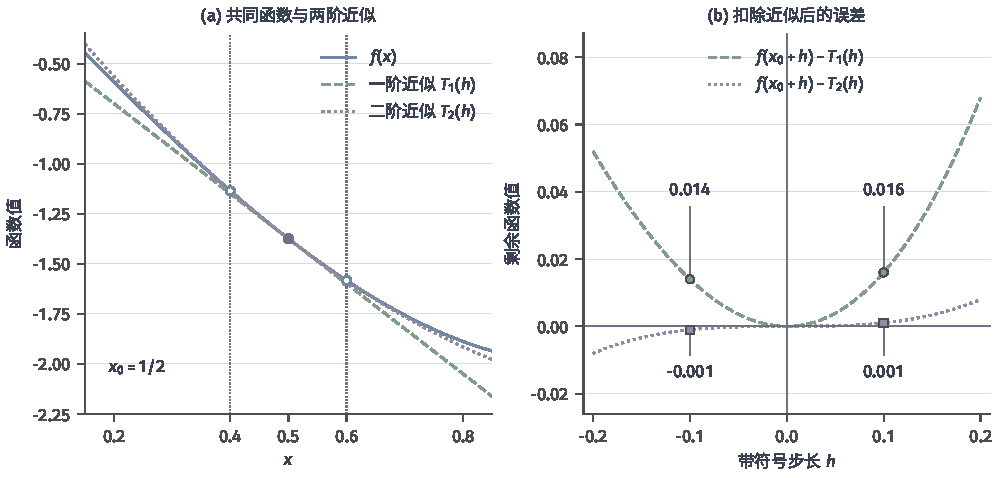
\includegraphics[width=169.0mm]{figures/01-mathematical-preliminaries-upper/01-mathematical-language-combinatorics-analysis-optimization/matplotlib/analysis-derivative-orders/figure.pdf}
 \caption{$f(x)=x^3-3x$在$x_0=1/2$处的Taylor近似，$h=x-x_0$。左图比较原函数、切线近似$T_1$与二次近似$T_2$；右图给出相应的带符号余项$3h^2/2+h^3$和$h^3$。标记点对应$h=\pm0.1$，余项的正负说明真值位于近似值的哪一侧。}
 \label{fig:analysis-derivative-orders}
\end{figure*}

\subsubsection{Peano余项}
如果只关心位移趋于零时误差的阶，可以不保留中间点，改用小量记号描述余项。
若$r\geq1$，$f$在包含$x_0$的某个开区间上属于$C^r$，则$h\to0$时
\[
 f(x_0+h)=\sum_{k=0}^r\frac{f^{(k)}(x_0)}{k!}h^k+o(|h|^r),
\]
称为带Peano余项的$r$阶Taylor公式。

推导时，对$r-1$阶Taylor公式使用Lagrange余项（这时定理~\ref{thm:analysis-taylor-lagrange}只要求$C^r$），得到$f(x_0+h)=T_{r-1}(x_0+h)+f^{(r)}(\xi_h)h^r/r!$，其中$\xi_h$位于$x_0$与$x_0+h$之间。把末项写成$f^{(r)}(x_0)h^r/r!$与$[f^{(r)}(\xi_h)-f^{(r)}(x_0)]h^r/r!$之和：前者与$T_{r-1}(x_0+h)$合成$T_r(x_0+h)$；后者除以$|h|^r$后趋于零，因为$\xi_h\to x_0$且$f^{(r)}$连续。这样就得到上式。

Peano余项描述局部误差的阶；若需要有限位移下的具体误差界，应使用Lagrange余项。$r=1$时上式就是式~\eqref{eq:analysis-scalar-first-order}，不过式~\eqref{eq:analysis-scalar-first-order}只需要$f$在该点可导。

\subsection{驻点的二阶导数判别}
在驻点处，Taylor公式的一阶项为零，函数在附近的增减就由二阶项决定。
设$a$是$f$的驻点，$f$在包含$a$的某个开区间上属于$C^2$。带Lagrange余项的一阶Taylor公式给出
\[
 f(a+h)-f(a)=\tfrac12f''(\xi_h)h^2,
\]
其中$\xi_h$位于$a$与$a+h$之间。若$f''(a)>0$，由$f''$的连续性，$h$充分小时$f''(\xi_h)\geq f''(a)/2>0$，所以每个充分小的非零$h$都使函数值严格增加，$a$为严格局部极小点。$f''(a)<0$时同理，$a$为严格局部极大点。

反之，在上述$C^2$条件下，局部极小点必须有$f''(a)\geq0$：若$f''(a)<0$，上一段说明$a$是严格局部极大点，附近其他点的函数值都严格小于$f(a)$，与局部极小矛盾。同理，局部极大点必须有$f''(a)\leq0$。

$f''(a)=0$时判别法没有结论：只知道前两阶导数，无法区分极小、极大与非极值。
\begin{example}[二阶导数为零时无法判别]
\label{ex:analysis-second-derivative-test-inconclusive}
考虑$x^4$、$-x^4$与$x^3$。三者在原点的一阶、二阶导数都为零：$(x^4)'=4x^3$、$(x^4)''=12x^2$，$(x^3)'=3x^2$、$(x^3)''=6x$，$-x^4$的导数只差一个符号。可是$x\neq0$时$x^4>0$，所以$0$是$x^4$的严格局部极小点；同理，$0$是$-x^4$的严格局部极大点；示例~\ref{ex:analysis-fermat-condition-failures}已说明$0$不是$x^3$的极值点。
\end{example}
回到示例~\ref{ex:analysis-cubic-stationary-points}，$f(x)=x^3-3x$有$f''(x)=6x$，$f''(1)=6>0$、$f''(-1)=-6<0$。二阶判别同样给出$1$为严格局部极小点、$-1$为严格局部极大点，与一阶导数判别的结论一致。

\FloatBarrier
